\section{问题的背景与重述}

\subsection{背景分析}

无人驾驶飞机是一种轻型、便捷、有动力、控制性强、能携带多种任务设备、 执行多种任务, 并可以重复使用的无人驾驶航空器[1]。其英文缩写为UAV中文简称为无人机。无人机早在二十世纪中期就已经在美国等地被初步研究,到了二十世纪末才得以在国际上掀起对无人机深度研究和广泛应用的热潮。而到了现在,无人机与人工自能相结合开发出了新的航空应用领域,其应用领域从最初的侦察、早期预警等军事领域广泛衍生到气象观测、资源勘测及处理突发事件等非军事领域[2]。无人机的引入对我国在军事方面加强的同时,也对我国日常生活中的应用带来了便捷。综上所述,无人机的引入使用对我国科学前言的研究具有重大意义。

\begin{figure}
    \centering
    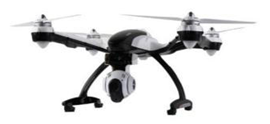
\includegraphics[scale=0.7]{../res/droneModel.png}
    \caption{无人机实体模型}
\end{figure}

\subsection{目标任务}

无人机的使用一般是群体联动进行作业,从而达到具有完成高强度任务的有利条件。无人机群在群体作业时为了防止外界对其干扰,机群内应尽可能保持电磁静默状态,少向外发射电磁波信号。同时,为了保持无人机之间相对位置的稳定,应建立相对应的定位模型使得无人机群在整体布局上呈现出无偏差效果,进而达到工作上的要求。

本文解决的主要问题是在无人机基于自身感知信息保持在同一个高度上飞行,由多个约束递进关系最终建立无人机群体联动作业的纯方位无源定位模型。

\subsection{问题重述}

问题1:在编队由十架无人机组成圆形编队,其中有九架无人机(编号FY01~FY09)均匀分布在同一高度的平面圆上,而另一架无人机(FY00)则位于圆心处。

\begin{figure}[h]
    \centering
    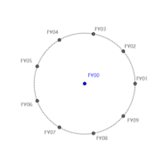
\includegraphics[scale=0.7]{../res/circleFormation.png}
    \caption{圆形无人机群编排图示}
\end{figure}

(1):处于圆心的无人机(FY00)与圆上的另外两架无人机为信号发射,其余无人机在略有偏差的位置被动接受信号。以发射信号的三架无人机组成无偏差的信号源区域,建立无人机群的定位模型。

(2):起初由编号FY00与FY01的无人机发射信号,而某位置略有偏差的无人机接受该两架无人机信号时也在接受若干编号的无人机发射的信号。若最后实现无人机的有效定位另还需要几架无人机发射信号。

(3):依编队约束,一架无人机位于圆心,另外九架无人机均匀分布在以半径为100m的圆周上。当初始时刻无人机位置有偏差时,给出相应合理的调整方案。具体数据参考如下:

\begin{tabular}{cc|cc}
    \toprule
    无人机编号& 极坐标(m,°)&  无人机编号& 极坐标(m,°)\\
    \midrule
    0&(0,0)&5	&(98,159.86)\\

    1	&(100,0)&	6&	(112,199.96)\\
    
    2	&(98,40.10)&	7	&(105,240.07)\\
    
    3	&(112,80.21)&	8	&(98,280.17)\\
    
    4	&(105,119.75)&	9&	(112,320.28)\\
    \bottomrule
\end{tabular}

问题2:在实际情况中,无人机也可为非圆形编队。若在锥形编队队形且考虑纯方位无源定位的情形设计出无人机位置的调整方案。模型图如下:

\begin{figure}
    \centering
    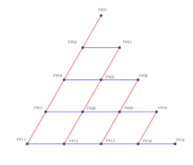
\includegraphics[scale=0.7]{../res/regularTriangleFormation.png}
    \caption{正锥形无人机编排图示}
\end{figure}


%%%%%%%%%%%%%%%%%%%%%%%%%%%%%%%%%%%%%%%%%%%%%%%


\section{问题分析}

\subsection{问题(1)的分析}

问题1(1)是十架无人机均匀分布在同一高度的某一圆周上,即编号FY00无人机与圆上相邻的两无人机夹角为 ,基于其中三架无人机为发射信号源建立定位模型的问题。
在该题中,题意明确,结合题意可知该模型是一个间接性二维平面模型,需要结合有关圆及三角函数知识联系坐标系建立相应的数学方程。
经过简单分析和几何关系可知,为了更好的表示几何关系,使最后呈现的模型可视化,将无人机群建立在空间直角坐标系中。
结合题设实际应用可知,被动接受信号的无人机是略有偏差的,故此所建立的模型过程中可引入偏差 。
本题将无人机群均匀分布在同高度的圆周平面上转化为理想的空间平面,利用空间直角坐标径向伸缩的幅度变化,通过建立多元非线性方程为目标函数,最终得到该无人机群的定位模型。
该小题的分析思路见下图。

问题一(1)分析思路流程图

\subsection{问题(2)的分析}

问题(2)在问题(1)的基础上,通过若干未知编号的信号发射无人机来实现无人机群有效定位的问题。
为了使问题较为可视化,将引入引理以及一个新的概念模型——\textbf{三圆定位模型}。
由题意确定发射信号无人机轨迹圆以及接收信号无人机偏离位置的轨迹圆建立坐标系,当接收信号无人机偏离位置的轨迹圆增加后,利用轨迹圆的大小及位置变化,通过联立圆的一般方程,并结合已知条件的应用,最终确定添加信号发射无人机的数量为两架。

\subsection{问题(3)的分析}

该问题要求以其中一架无人机位于圆心,另九架无人机均匀分布在半径为$100m$的圆周上,且要求整个无人机群中最多有四架无人机是可发射信号的。由表一给出的无人机初始位置数据可知,结果的圆是以编号$00$的无人机为圆心,与之相距$100m$的$01$编号无人为半径的圆。故此两圆是初始位置的参考圆,也是最后所要调整的目标圆。若仅根据接受到的方向信息调整无人机的位置,可以通过建极坐标系确定表一上无人机最初的位置。对表一的数据进行预处理,计算发现角度偏差在$0.01 \thicksim 0.02$之间,对其用极坐标方程列出各无人机的位置关系进行模拟调整,进而重复操作得到最终的编队要求。


%%%%%%%%%%%%%%%%%%%%%%%%%%%%%%%%%%%%%%%%%%%%%%%


\section{模型假设}

为了适当对模型进行合理简化,故作出以下假设:

\begin{itemize}
    \item 假设模型中所有无人机接受信号的时间一致
    \item 假设无人机在实体模型的建立中不受外界因素影响
    \item 假设模型建立过程中所使用的无人机为理想型且型号一致
\end{itemize}


%%%%%%%%%%%%%%%%%%%%%%%%%%%%%%%%%%%%%%%%%%%%%%%


\section{符号说明}

\begin{table}[ht]
\centering
\begin{tabular}{ccc} 
    \hline
    \Large 符号 & \Large 说明 & \Large 单位 \\
    \hline

    $\rho$ & 表示极径 & 有量纲(长度) \\
    $\alpha$ & 表示距离 & 度(°) \\
    $r$ & 表示距离 & 有量纲(长度) \\
    $\varepsilon_{\rho i}$ & 表示偏差 & 有量纲(长度) \\
    $\Delta x_i$ & 表示地址偏差 & 有量纲(长度) \\
    $\sigma^2_\rho$ & 表示方差 & 无量纲 \\
    $l$ & 表示长度 & 有量纲(长度) \\
    $R$ & 表示半径 & 有量纲(长度) \\
    $k$ & 表示斜率 & 无量纲 \\
    $\lambda$ & 表示距离 & 有量纲(长度) \\
    $\alpha$ & 表示变量 & 无量纲 \\
    $A$、$B$ & 表示矩阵 & 无量纲 \\
    $H_y$ & 表示方程解 & 无量纲 \\
    $y_{Tu}$ & 表示定位解 & 无量纲 \\
    $G_i(i=1,2,3,4)$ & 表示代数矩阵 & 无量纲 \\
    $x$、$y$、$z$ & 表示坐标代数距离 & 无量纲 \\
    $y$ & 表示初步定位解 & 无量纲 \\
    $O_i$ & 表示圆心 & 无量纲 \\
    $\rho_i$ & 表示矩阵 & 无量纲 \\

    \hline 
\end{tabular}
\end{table}